\section{Empirical Study Design}
\label{sec_empirical_study}

We perform two complementary studies: one quantitative and one qualitative. For each study, we describe their studied projects, their data collection process, and their methodology.

\subsection{\textbf{Quantitative Study---Study I}}
\label{sec_quantitative_study}

In Study I, we divide our projects in two time periods, \textit{before} and \textit{after} the adoption of \textsc{TravisCI}. Segmenting the data into these two time periods is necessary to study the association between the adoption of \textsc{TravisCI} and the delivery time of PRs.

\subsubsection{Studied Projects}
\label{subsec_quant_studided_projects}

Our goal is to identify projects with substantial historical data that adopted \textsc{TravisCI} eventually. We use such projects to better understand the potential influence of adopting a CI service on the delivery time of merged PRs. We use an approach similar to \cite{Vasilescu2015-tn} and \cite{Hilton2016-xy} to select projects that use \textsc{TravisCI}. We use the date of the first build on \textsc{TravisCI} to determine when \textsc{TravisCI} was introduced in a project. 

We selected a set of 87 popular \textsc{GitHub} projects (33 JavaScript, 23 Python, 11 Java, 10 Ruby, and 10 PHP). We collect metrics related to the PRs and releases of each project. 
The detailed information about all computed metrics for each PR is described in Tables \ref{tab_explanatory_variables_1} and \ref{tab_explanatory_variables_2}. We believe these metrics can be correlated with the \textit{delivery time} of merged PRs. A total of 162,653 delivered PRs were collected (123,543 PRs were delivered \textit{after} the adoption of \textsc{TravisCI}, whereas 39,110 were delivered \textit{before} the adoption of \textsc{TravisCI}). The unbalanced number of PRs across time periods is a reflection of the duration of the adoption of \textsc{TravisCI} in different projects. The median age of our projects is 5.1 years, where the use of \textsc{TravisCI} accounts for 60.8\% (3.1 years) of the age of our projects. Table \ref{tab:pulls_per_language} shows the number of PRs per programming language \textit{before} and \textit{after} the adoption of \textsc{TravisCI}. Our project selection and data collection processes are explained in more detail in an earlier publication of this work \citep{bernardo2018studying}.

\bgroup
\def\arraystretch{1.1}
\begin{table}[t]
	\centering
	\footnotesize
	\caption{Summary of the number of projects and released pull requests grouped by programming language.}
	%\rowcolors{1}{}{lightgray}
	\begin{tabular}{|c|c|c|c|c|}
		\hline
		\textbf{Language} & \textbf{Projects} & \textbf{PRs total}  & \textbf{PRs \textit{before} CI} & \textbf{PRs \textit{after} CI} \\
		\hline \hline
		JavaScript   & 33 & 57,104  & 17,556 & 39,548  \\ 
		Python       & 23 & 55,003 & 9,107 & 45,896  \\ 
		Java           & 11 & 7,700   & 3,433 & 4,267    \\ 
		Ruby          & 10 & 22,864 & 3,197 & 19,667  \\ 
		PHP            & 10 & 19,982 & 5,817 & 14,165  \\ 
		\hline
		\textbf{Total} & \textbf{87} & \textbf{162,653}  & \textbf{39,110} & \textbf{123,543} \\ 
		\hline
	\end{tabular}
	\label{tab:pulls_per_language}
\end{table}
\egroup

\bgroup
\def\arraystretch{1}

\begin{table*}[htbp]
	\caption{Metrics that are used in our explanatory models (resolver, pull request, and project dimensions).}
	\footnotesize
	\begin{tabular}{|>{\centering\arraybackslash}m{0.45in}|m{0.60in}|m{0.4in}|m{2.5in}|}
		\hline
		\textbf{Dimension} & \textbf{Attributes} & \textbf{Type} & \textbf{Definition (d) | Rationale (r)} \\ \hline
		\multirow{12}{*}{Resolver} & \multirow{7}{2cm}{Contributor Experience}
		& \multirow{7}{*}{Numeric} & \textbf{d:} The number of
		previously released PRs that were submitted by the contributor of a
		particular PR. We consider the author of the PR to be its
		contributor. \\ \cline{4-4}
		& &  & \textbf{r:} The greater
		the experience and participation of a user within a specific
		open-source project, the greater his/her chance of having
		his/her PR reviewed and integrated into the codebase of such a project
		by its core integrators \citep{shihab2010predicting}.   \\
		\cline{ 2- 4}
		
		& \multirow{5}{2cm}{Contributor Integration} & \multirow{5}{*}{Numeric} & \textbf{d:} The average in days of the previously released PRs that were submitted by
		a particular contributor.
		\\ \cline{4-4}
		& &  & \textbf{r:} If a particular contributor usually submits PRs that are merged and released quickly, his/her future PR might be merged and released quickly as well \citep{Da_Costa2016-cb}.  \\ \hline
		
		% pull-request
		
		\multirow{11}{1.2cm}{Pull Request} & \multirow{6}{2cm}{Stack Trace Attached} & \multirow{6}{*}{Boolean} & \textbf{d:} We verify if the PR report has a stack trace attached in its description. \\ \cline{4-4}
		& &  & \textbf{r:} 
		If the PR provides a bug fix, a stack trace attached may provide useful information regarding the causes of the bug and the importance of the submitted code, which may quicken the merge of the PR and its delivery in a release of the project \citep{schroter2010stack}.\\ \cline{ 2- 4}
		& \multirow{4}{1.5cm}{Description Size} & \multirow{4}{*}{Numeric} & \textbf{d:} The number of characters in the body (description) of a PR.
		\\ \cline{4-4}
		& &  & \textbf{r:} PRs that are well described might be easier to merge and release than PRs that are more difficult to understand  \citep{Da_Costa2016-cb}.
		\\ \hline
		
		% project
		
		\multirow{13}{*}{Project} & \multirow{4}{2cm}{Queue Rank} & \multirow{4}{*}{Numeric} & \textbf{d:} The number that represents the moment when a PR is merged compared to other merged PRs in the release cycle. For example, in a queue that contains 100 PRs, the first merged PR has position 1, while the last merged PR has position 100.  \\ \cline{4-4}
		& &  & \textbf{r:} A PR with a high \textit{queue rank} is a recently merged PR. A merged PR might be released faster/slower depending on its queue position \citep{Da_Costa2016-cb}. \\ \cline{ 2- 4}
		
		& \multirow{6}{1.5cm}{Merge Workload} & \multirow{6}{*}{Numeric} & \textbf{d:} The number of PRs that were created and still waiting to be merged by a core integrator at the moment at which a specific PR is submitted. \\ \cline{4-4}
		& &  & \textbf{r:} A PR might be released faster/slower depending of the
		amount of submitted PRs waiting to be merged. The higher the
		amount of created PRs waiting to be analyzed and merged, the
		greater the workload of the contributors to analyze these PRs,
		which may impact their delivery time.
		\\ \hline
	\end{tabular}
	\label{tab_explanatory_variables_1}
\end{table*}
\egroup

\bgroup
%	\def\arraystretch{1.2}
\def\arraystretch{1}

\begin{table*}[htbp]
	\caption{Metrics that are used in our explanatory models (process dimension).}
	\footnotesize
	\begin{tabular}{| >{\centering\arraybackslash}m{0.45in}|m{0.60in}|m{0.4in}|m{2.5in}|}			
		\hline
		\textbf{Dimension} & \textbf{Attributes} & \textbf{Type} & \textbf{Definition (d) | Rationale (r)} \\ \hline
		
		\multirow{33}{*}{Process} & \multirow{4}{2cm}{Number of Impacted  Files} & \multirow{4}{*}{Numeric} & \textbf{d:} The number of files linked to a PR submission.  \\ \cline{4-4}
		& &  & \textbf{r:} The delivery time might be related to the high number of files of a PR, because more effort must be spent to integrate it \citep{jiang2013will}.   \\ \cline{ 2- 4}
		
		& \multirow{5}{*}{Churn} & \multirow{5}{*}{Numeric} & \textbf{d:} The number of added lines plus the number of deleted lines to a PR.
		\\ \cline{4-4}
		& &  & \textbf{r:} A higher churn suggests that a great amount of work might be required to verify and integrate the code contribution sent by means of PR \citep{jiang2013will, nagappan2005use}.  \\ \cline{ 2- 4}
		
		& \multirow{3}{*}{Merge Time} & \multirow{3}{*}{Numeric} & \textbf{d:} Number of days between the submission and merge of a PR.
		\\ \cline{4-4}
		& &  & \textbf{r:} If a PR is merged quickly, it is more likely to be released faster.  \\ \cline{ 2- 4}
		
		& \multirow{5}{2cm}{Number of Activities} & \multirow{5}{*}{Numeric} & \textbf{d:} An activity is an entry in the PR's history. 
		\\ \cline{4-4}
		& &  & \textbf{r:} A high number of activities might indicate that much work was required to make the PR acceptable, which may impact the integration of such PR into a release \citep{jiang2013will}.  \\ \cline{ 2- 4}
		
		& \multirow{5}{2cm}{Number of Comments} & \multirow{5}{*}{Numeric} & \textbf{d:} 
		The number of comments of a PR.  \\ \cline{4-4}
		& &  & \textbf{r:} A high number of comments might indicate the
		importance of a PR or the difficulty to understand it
		\citep{giger2010predicting}, which may impact its delivery time \citep{jiang2013will}. \\ \cline{ 2- 4}
		
		& \multirow{5}{2cm}{Interval of Comments} & \multirow{5}{*}{Numeric} & \textbf{d:} 
		The sum of the time intervals (days) between comments divided by the total number of comments of a PR.   \\ \cline{4-4}
		& &  & \textbf{r:} A short \textit{interval of comments} indicates the discussion was held with priority, which suggests that the PR is important, thus, the PR might be delivered faster \citep{Da_Costa2016-cb}. \\ \cline{ 2- 4}
		
		& \multirow{5}{1.5cm}{Commits per PR} & \multirow{5}{*}{Numeric} & \textbf{d:} Number of commits per PR.
		\\ \cline{4-4}
		& &  & \textbf{r:} The higher the number of commits in a
		PR, the greater the amount of contribution to be analyzed by the project integrators, which might impact the delivery time of the PR.  
		\\ \hline
	\end{tabular}
	\label{tab_explanatory_variables_2}
\end{table*}
\egroup

\subsubsection{Research Approach}

Figure \ref{fig_released_pull_request_life_cycle} shows the basic life cycle of a delivered PR, where $t1$ is the merge phase and $t2$ is the delivery phase. We refer to  $t1 + t2$ as the lifetime of a PR. In $RQ1$, we analyze the \textit{merge} and \textit{delivery} phases. The merge phase ($t1$) is the required time for PRs to be merged into the codebase, whereas the \textit{delivery phase} ($t2$) refers to the required time for merged PRs to be released. 

\begin{figure}[t]
	\centering
	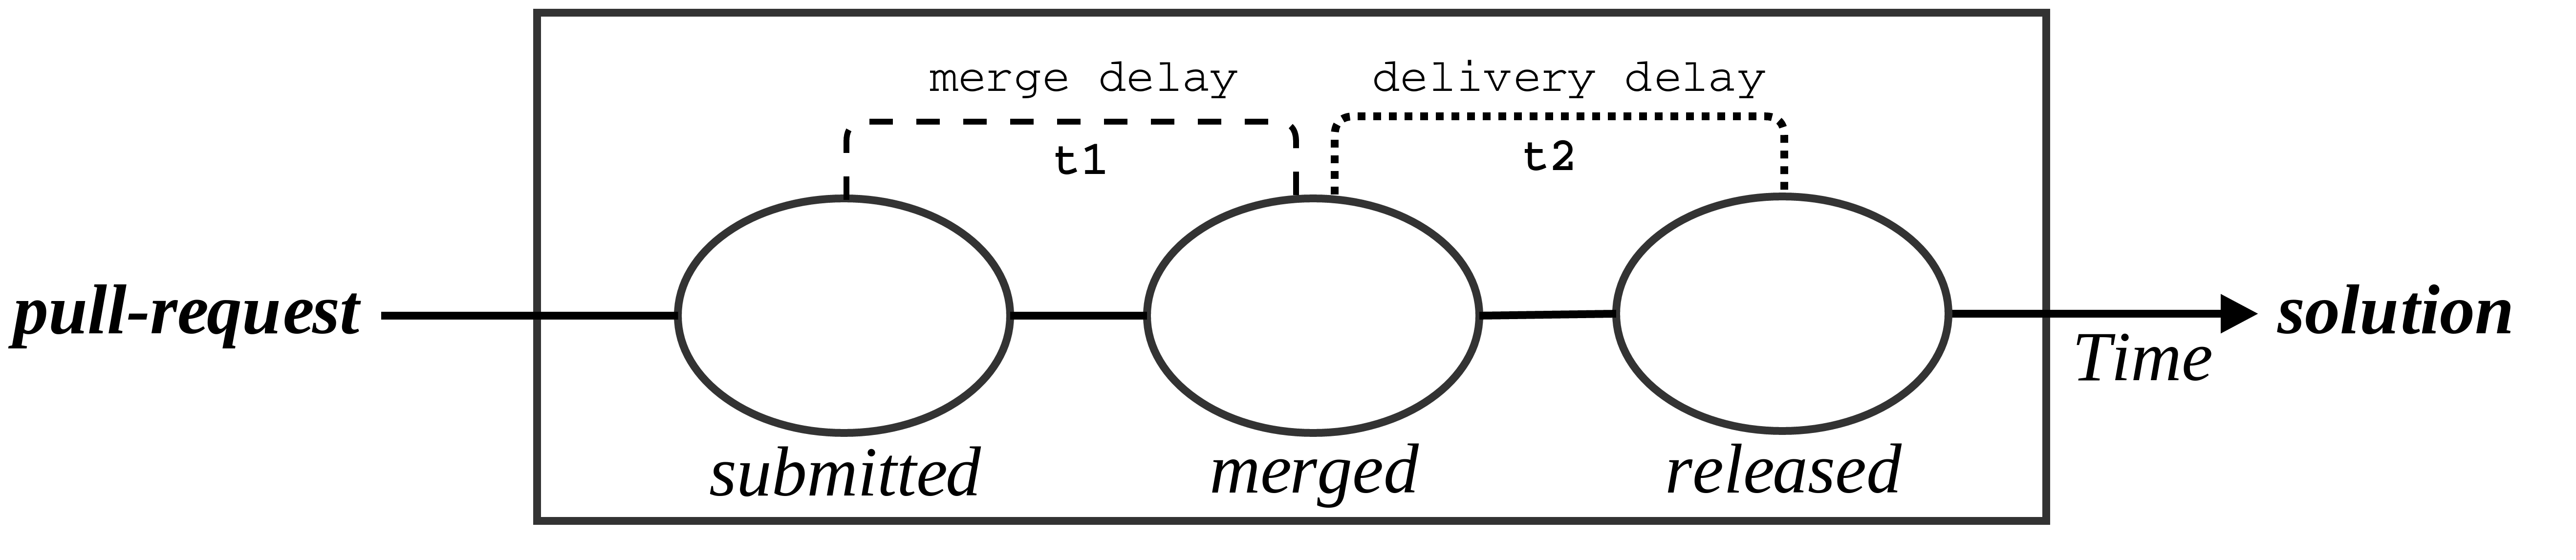
\includegraphics[width=\columnwidth,keepaspectratio]{released_pull_request_life_cicle_2.png}
	\caption{The basic life-cycle of a delivered pull request.}
	\label{fig_released_pull_request_life_cycle}
\end{figure}


We use Mann-Whitney-Wilcoxon (MWW) tests~\citep{wilks2011statistical} and Cliff's delta effect-size measurements~\citep{cliff1993dominance} to compare different distributions of values. MWW is a non-parametric test whose null hypothesis is that two distributions come from the same population ($\alpha = 0.05$). The Cliff's delta is a non-parametric effect-size metric to verify the magnitude of the difference between the values of two distributions. 
%The higher the Cliff's delta value, the greater the difference between distributions. A positive Cliff's delta shows how much larger are the values of the first distribution, while a negative Cliff's delta shows the opposite. 
We use the thresholds provided by \citet{Romano:2006} to interpret the Cliff's delta, i.e. $delta<0.147$ (\textit{negligible}), $delta<0.33$ (\textit{small}), $delta<0.474$ (\textit{medium}), and $delta>=0.474$ (\textit{large}). We analyze the entire life-cycle of a PR \textit{before} and \textit{after} the adoption of \textsc{TravisCI}. First, we analyze the \textit{delivery time} ($t2$) and then, we analyze the {\em merge time} ($t1$). Lastly, we analyze the {\em lifetime} of a PR ($t1 + t2$).

Similar to $RQ1$, in $RQ2$ we use MWW tests \citep{wilks2011statistical}
and Cliff's delta measurements \citep{cliff1993dominance} to analyze the data. We use
box plots \citep{Williamson-1989} to visually summarize the distributions and perform comparisons.
In $RQ2$, we investigate whether the increase in the lifetime of PRs
\textit{after} adopting \textsc{TravisCI} is related to a significant increase in PR
submission, merge, and delivery rates (also \textit{after} the adoption of \textsc{TravisCI}). 

We group our dataset into two time periods: \textit{before} and \textit{after} the
adoption of \textsc{TravisCI}. For each time period, we count the number of PRs that are submitted,
merged, and delivered per release.  We perform three comparisons in $RQ2$.
First, we compare whether the PR submission, merge, and delivery rates per
release significantly increase \textit{after} the adoption of \textsc{TravisCI}. Next, we verify
whether there is a statistical increase in the release frequency of the
projects \textit{after} the adoption of \textsc{TravisCI}. 
%A high increase or decrease in the release frequency may lead to an increase or decrease in the PR delivery rate per release, once the release size changes. 
We use the Pearson correlation \citep{best1975algorithm},
to test whether two variables are significantly correlated. 
%The {\em Correlation Coefficient} (CC) between two variables is comprised between $-1$ and $1$. A CC of $-1$  indicates a strong negative correlation, i.e., every time $x$ increases, $y$ decreases. A CC of $0$ indicates no correlation between the two variables, while $1$ indicates a strong positive correlation, i.e., when $x$ increases, $y$ also increases. 

In RQ3, we use multiple regression modeling ({\em Ordinary Least Squares}) to describe the
relationship between $X$ (i.e., the set of explanatory variables, e.g.,
\textit{churn}, \textit{description length}), and the response variable $Y$,
i.e., the \textit{delivery time} of merged PRs in terms of days. We control
covariates that might influence the results. For each project, we build two
explanatory models, one using the PR data \textit{before} the adoption of \textsc{TravisCI}, and another using
PR data \textit{after} the adoption of \textsc{TravisCI}. Tables \ref{tab_explanatory_variables_1} and \ref{tab_explanatory_variables_2} show the definition and rationale for each explanatory variable used in our
models. Our response variable $Y$ is the length of time between when a PR was merged and the time at which the same PR was delivered (i.e., delivery time).

We follow the guidelines of \citet{harrell2015regression} for fitting linear models.  We assess how stable our models are by computing the \textit{optimism-reduced} $R^2$. Finally, we use the Wald $X^2$ maximum likelihood test to evaluate the impact of each explanatory variable in our models. The larger the $X^2$ value for a variable, the larger the impact of a variable \citep{Da_Costa2016-cb}.
Next, we analyze the direction of the relationship between the most influential variables of our models and the delivery time. 
%To do this, we use the \textit{Predict} function of the \textit{rms} package of the \textsf{R} language to plot the change in the delivery time against the change in each impactful variable while holding the other variables constant at their median values. 
The process we use to build our statistical models is explained in more detail in our earlier publication~\citep{bernardo2018studying}.

\subsection{\textbf{Qualitative Study (Study II)}}
\label{sec:qualitative_study}

In this section, we explain the data collection and research approach of our qualitative study (Study II).

\subsubsection{Subject Projects}
\label{sec:subject_projects}

As the main goal of qualitative analysis is to complement Study I, we select the same 87 GitHub projects used in Study I for Study II. 
The goal of Study II is to better understand the influence CI can have on the delivery time of merged PRs.
We also take the opportunity to better understand the perceived influence of CI on the code review and release processes of our studied projects (i.e., according to the perception of our participants).

\subsubsection{Data Collection}
\label{sec:data_collection}

We first identify contributors who have submitted at least one PR that made into an official release of their project. The release date of the PRs must have fallen between the projects' creation date and November 11th, 2016, i.e., the range used in our search on \textsc{GitHub} for Study I. By inspecting the PR meta-data of the studied projects, we find a total of 20,698 contributors that fulfill our criteria. To prioritize frequent contributors, for each studied project, we select 15\% of contributors that have the highest number of delivered PRs, resulting in 3,105 contributors.

To collect our data, we designed a web-based survey and sent it by email to all 3,105 participants (i.e., the contributors of our subject projects). To encourage participation, we randomly provided six \$50 Amazon gift cards to respondents who explicitly stated their willingness to participate in the draw. To be eligible for the gift cards, the participants needed to answer all questions of the survey. In total, we received 450 responses, resulting in a response rate of 14.5\% (\nicefrac{450}{3105}). Our invitation letter is available in Appendix~\ref{sec:appendix_invitation_latter}.

Our survey has three major \textit{parts}. The first part concerns the influence of CI on the delivery time of merged PRs, whereas the second and third parts concern the potential influence of CI on the release and review processes of the studied projects, respectively. A complete example of our survey is available in Appendix \ref{sec:appendix_project_survey_example}, which shows the questionnaire sent to participants of the \textit{haraka/haraka}\footnote{\url{github.com/haraka/haraka}} project. Because our goal was to provide data specific to the projects of our participants, we designed 87 different questionnaires, aiming to obtain richer information about the project and encourage participants to respond more fully to the survey.

Our questionnaire is organized as follows. The first six questions (\#3--\#8) collect demographic information. Questions \#9--\#13 tap into the general experience of our participants, whereas questions \#14--\#26 present data specific to our participants' projects. 
In terms of questions' goals, questions \#9--\#13 and \#26 capture the potential influence of CI on the delivery time of merged PRs. 
\textit{Question \#14} captures the perceived correctness of our approach to define the \textsc{TravisCI} adoption date in our studied projects. 
\textit{Questions \#17--\#21} capture the potential influence of CI on the code review process of the projects, whereas \textit{Questions \#22--\#25} capture the potential influence of CI on the release process of the projects. 

\subsection{Research Approach}
\label{sec:research_approach}

We use an inductive thematic analysis, which is designed for identifying, analyzing, and reporting themes found within qualitative data~\citep{braun2006using}. In this study, we use the guidelines proposed by \cite{nowell2017thematic} to perform our thematic analysis.

The first step in our thematic analysis is the coding of our data. This step consists of attaching codes to any piece of relevant qualitative data collected from our questionnaire. The first author conducts three sessions of open coding of the responses to open-ended questions. The second author independently conducts three sessions of open coding for 10\% of the responses for each of those questions. Afterward, a new set of codes is generated by the merge of the codes created by each author. 
We use Cohen's Kappa test to verify the agreement rate between authors when coding the responses to 13 open-ended questions of our questionnaire.
We calculate the Kappa value separately for each of the 13 questions. We achieved a median Kappa value of 0.84, indicating substantial agreement~\citep{landis1977kappa}. 
The third author reviews the set of codes to add additional entries and resolve disagreements between the codes from the first and second authors. 
Next, the first author organizes the codes into {\em themes} through axial coding. These themes represent higher conceptual constructs (e.g., a theme might group many codes). 
This categorization was double-checked by the second author. 
We report the codes and themes generated by our thematic analysis in the result section. When reporting the results of $RQ4$---$RQ8$, we indicate (in superscript) the number of quotes citing each code and theme. It is important to highlight that the number in superscript does not necessarily indicate the relevance of a code, e.g., a code may be mentioned in more quotes because the code is more easily remembered by our participants. 
Additionally, when reporting our qualitative results, the frequency with which codes occur across responses can be higher than the total of responses. This is because a response from a participant can be associated with several codes. For example, consider the following quote \textit{``Anything that is considered a critical security fix or major bug fix is generally shipped within 1-2 weeks of submission. This happens frequently"} (C020). We derived two codes from this quote, which are \textit{bug fix} and \textit{security fix}.
We use representative quotes from our participants to aid in the understanding of the interpretation of the codes. 
We omit the participants' names by replacing them with an ID, e.g., {\em participant 01} receives the ``name'' C001. In Appendix \ref{sec:appendix_participants_ids_and_their_projects}, we provide the IDs assigned to our participants and their project. 

